\documentclass[a4paper]{report}
\usepackage{amsmath}
\usepackage{blindtext}
\usepackage{blindtext}
\usepackage[utf8]{inputenc}
\usepackage{graphicx}
\usepackage{appendix}


\usepackage{caption}
\usepackage{subcaption}

%front page:
\usepackage[T1]{fontenc}
\usepackage{xcolor}

%for MATLAB code:
\usepackage[framed,numbered,autolinebreaks,useliterate]{mcode}

\usepackage{geometry}
\geometry{a4paper, margin=1in}


\begin{document}
	
\begin{titlepage}

		\centering
		\vspace*{5\baselineskip}
		\Huge
		\textbf{Finite Elements}
		\\[2\baselineskip]
		\normalsize
		Rick Koster\\
		Ruben Termaat\\
		\today
		\vfill
		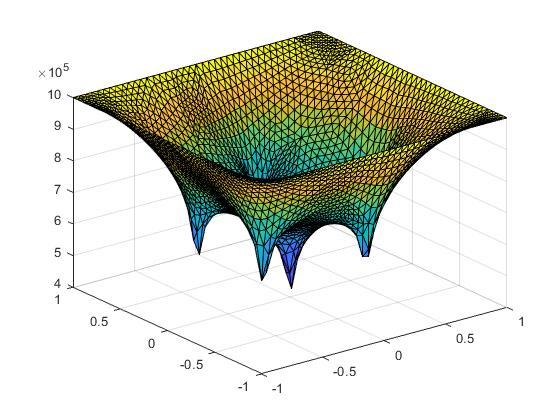
\includegraphics[width=15cm]{3Dv.jpg}
		\vfill
	
\end{titlepage}
	
\clearpage\mbox{}\clearpage



\chapter*{Preface}
\addcontentsline{toc}{chapter}{\protect\numberline{}Preface}
This report was written in order to better understand and demonstrate how one can apply finite elements in combination with MATLAB. Solving boundary value problem through finite elements will help engineers understand difficult dynamics of systems.To show this first a general 1D problem with boundary conditions is presented, solved and computed. Secondly a real life problem is presented, where the flow velocity and pressure within a square reservoir for water filtration is calculated. This is done by solving the boundary value problem of a square reservoir of domain  $\Omega= (-1; 1) \times (-1; 1)$ and its boundary conditions, then adapting the 1D MATLAB code to this 2D case and finally computing and plotting velocity flow charts and a 3D surface plot.


\clearpage\mbox{}\clearpage

\tableofcontents


\chapter{1D-case}



On the 1D interval of $x = [0,1]  $, we consider a steady-state convection-diffusion-reaction equation, with homogeneous Neumann boundary conditions. The following equations apply to this domain:

\begin{equation}
\begin{cases} 
-D\triangle u + \lambda u = f(x),\\ -D\frac{du}{dx}(0) = 0 ,\\ -D\frac{du}{dx}(1) = 0
\end{cases} 
\end{equation}
\bigskip

In this report $\triangle$ denotes the laplacian operator. The function f(x) is a given funtion, where D and $\lambda$ are positive real constants. In order to solve this boundary value problem (BVP), first the interval is divided in n-1 elements(n = positive integer). This results in the domain being divided in elements: $e_i = [x_i, x_{i-1}]$ where $i={1,2,..,n}$. 

In order to solve this BVP, the solutions for the given equations will first be calculated and then computed using MATLAB codes.


\section{Boundary value problem 1D}
\vspace{5mm}

In order to find the Weakform of the given equations(1.1), both sides are multiplied by a test function  $\phi(x)$ and then integrate both sides over the domain $\Omega$. In the equations  $\phi(x)$ is written as $\phi$


\begin{equation}
	 \int_{\Omega} \phi(-D\triangle u + \lambda u )d\Omega = \int_{\Omega} \phi f(x) d\Omega 
\end{equation}	
\smallskip

Now by rewriting and then using partial integration the following equation can be found:


\begin{equation}
	\int_{\Omega} (\nabla\cdot(-D\phi\cdot\nabla u) + D\nabla\phi\nabla u +\phi \lambda u) d\Omega = \int_{\Omega} \phi f(x) d\Omega 
\end{equation}
\smallskip

Applying Gauss on the first term on the left side of equation(1.3):


\begin{equation}
	\int_{\Omega}  \vec{n}\cdot(-D\phi \nabla u) d\tau + \int_{\Omega}  (D\nabla\phi\cdot\nabla u +\phi\lambda u )d\Omega = \int_{\Omega} \phi f(x) d\Omega 
\end{equation}
\smallskip

Using the boundary conditions from equations(1.1) the boundary integral equals to 0 and then the following weak formulation(WF) is found: \vspace{5mm}


(WF): \begin{equation}
\begin{cases} 
	$find u $\epsilon \sum =\{u$ $ smooth\}$ Such that:$ \\ \int_{\Omega}  (D\nabla\phi\cdot\nabla u +\phi\lambda u )d\Omega = \int_{\Omega} \phi f(x) d\Omega \\ \forall\phi $ $ \in\sum 
\end{cases}\  
\end{equation}

\bigskip
The next step is to substitute the Galerkin equations into the found diferential equation, where u is replaced by $ \sum_{j=1}^{n}c_i\phi_j $ and  $\phi(x)=\phi_i(x)$ with $i = [1,..,n]$. Filling this in equation (1.5) the following equation is found:

\begin{equation}
	\sum_{j=1}^{n}c_i\int_{0}^{1} (D\nabla\phi_i\cdot\nabla\phi_j +\lambda\phi_i\phi_j )d\Omega = \int_{0}^{1} \phi_i f(x) d\Omega
\end{equation}
\medskip

Which is of the form of $ S\vec{c} = \vec{f} $

\section{Element matrix}\label{Element_matrix}
Now the found Galerkin equations can be used to compute $ S_{ij}$  the element matrix, over a generic line element $ e_i$.

\begin{equation}
S\vec{c}=	\sum_{j=1}^{n}c_i\int_{0}^{1} (D\nabla\phi_i\cdot\nabla\phi_j +\lambda\phi_i\phi_j )d\Omega
\end{equation}

\begin{equation}
S_{ij} =\sum_{l=1}^{n-1} S^{e_k}_{ij} 
\end{equation}
\medskip

Now to solve S we solve the following equation, over the internal line element.

\begin{equation}
S^{e_k}_{ij} = -D\int_{e_k}\nabla\phi_i\cdot\nabla\phi_j d\Omega+\lambda\int_{e_k}\phi_i\phi_j dx
\end{equation}


\section{Element vector}\label{Element_vector}
Again the found Galerkin Equations(1.6) are used in order to compute the element vector $f_i$ over a generic line-element.

\begin{equation}
f^{e_k}_i = \int_{e_k}\phi_i f dx
\end{equation}

\begin{equation}
	f^{e_k}_i =\frac{\lvert x_k-x_{k-1}\lvert}{(1+1+0)!}f(\vec{x}) =\frac{\lvert x_k-x_{k-1}\lvert}{2}
	\begin{bmatrix} f^{e_n}_{k-1}\\ f^{e_n}_{k}
	\end{bmatrix}
\end{equation}







\section{Boundary value problem 1D MATLAB routine}

\subsection{mesh and elmat code}
The first step in order to solve the BVP is to write a MATLAB routine that generates an equidistant distrubition of points over the given interval of $[0,1]$(generate a mesh with n-1 elements).

\begin{lstlisting}
	function [ x ] = GenerateMesh(int, N_elem)
	%GenerateMesh Creates a mesh for 1D problems
	
	x = linspace(int(1,1),int(1,2),N_elem);
	end
	
\end{lstlisting}
	
Using the codes to generate a mesh and the elmat, it is easier to use this 1D problem and adapt to a higher dimensional problem. The next step is to write a code that generates a two dimensional array, called the elmat.
\newpage
\begin{lstlisting}
	function [ elmat ] = GenerateTopology( N_elem )
	%GenerateTopology Creates the topology for a 1D problem given mesh 'x'.
	
	elmat = zeros(N_elem,2);
	elmat(i,1) = i;
	elmat(i,2) = i + 1;
	end

\end{lstlisting}

\subsection{Element matrix}

Now that the base MATLAB codes are made the element matrix and element vector codes can be written. The first step in this process is, is to compute the element matrix $S_{elem}$.

\begin{lstlisting}
	function [ Selem ] = GenerateElementMatrix( k, elmat, D, lambda, mesh)
	%GenerateElementMatrix Creates element matrix S_ek
		
	Selem = zeros(2,2);
	
	i = elmat(k,1);
	j = elmat(k,2);
	
	x1 = mesh(i);
	x2 = mesh(j);
	
	element_length = abs(x1-x2);
	
	slope = 1/element_length; 
	
	for m = 1:2
		for n = 1:2
			if m == n
				Selem(m,n) = element_length*((-1)^(abs(m-n))*D*slope^2
				+ (2)*lambda/6);
			else
				Selem(m,n) = element_length*((-1)^(abs(m-n))*D*slope^2
				+ (1)*lambda/6);
			end
		end
	end
	end
\end{lstlisting}

\bigskip




\subsection{Assemble matrix S}
To generate a n-by-n matrix S, the sum over the connections of the vertices in each element matrix, over all elements has to be calculated. The following code computes this matrix:

\begin{lstlisting}
	function [ S ] = AssembleMatrix( N_elem, int, lambda, D)
	% global N_elem 
	
	elmat = GenerateTopology(N_elem);
	
	S = zeros(N_elem,N_elem);
	
	for i = 1:N_elem-1
		Selem = GenerateElementMatrix(i, elmat, int, N_elem, D, lambda);
		for j = 1:2
			for k = 1:2
				S(elmat(i,j), elmat(i,k)) =
				S(elmat(i,j), elmat(i,k)) +	Selem(j,k);
			end
		end
	end
	end

\end{lstlisting}



All the previous code will generate a large matrix S, from the element matrices $S_{elem}$ over each element.\\



\subsection{Element vector MATLAB routine}

The next step In order to solve the equation $S\vec{c}=f$ is to create a code to generate the element vector. This element vector provides information about node $i$ and node $i+1$, which are the vertices of element $e_i$.\\



\begin{lstlisting}
	function [ felem ] = GenerateElementVector( i, elmat, mesh )
	%GenerateElementVector Creates element vector f_ek
	
	
	felem = [0;0];
	
	k1 = elmat(i,1);
	k2 = elmat(i,2);
	
	x1 = mesh(k1);
	x2 = mesh(k2);
	
	element_length = abs(x1-x2);
	
	felem = (element_length/2*arrayfun(@functionBVP,[x1,x2]))';
	
	end
\end{lstlisting}

Where the function $f(x)$ from the BVP is defined in the following function. The different definitions of $f(x)$ will be used in different assignments.

\begin{lstlisting}
function [f] = functionBVP(x)
f = 1;
%f = sin(20*x);
%f = x;
end
\end{lstlisting}

\smallskip

To generate the vector f, the sum over the connections of the vertices in each element matrix, over all elements $i\,\epsilon\, \{1,...,n-1\}$  has to be calculated. 

\bigskip

	
\begin{lstlisting}
	function [ f ] = AssembleVector( N_elem, int, lambda, D )
		
	f = zeros(N_elem,1);
	elmat = GenerateTopology(N_elem);
		
	for i = 1:N_elem-1
		felem = GenerateElementVector(i, elmat, int, N_elem);
		for j = 1:2
			f(elmat(i,j)) = f(elmat(i,j)) + felem(j);
		end
	end
\end{lstlisting}	




\subsection{Computing S and f}

Now if the previous MATLAB codes are run the following happens. First, a mesh and 1D topology are build. These are needed for the S matrix and f vector. The second step is to calculate the S matrix and f vector themselves through the found equations of section \ref{Element_matrix} and \ref{Element_vector}. The final step is to use the found matrix and vector to solve the equation $Su=\vec{f}$.





\section{Main program}

The main program is simply written by assembling the previous created MATLAB code AssembleMatrix and AssembleVector and deviding the vector f by the matrix S.
\begin{lstlisting}
	function [ u ] = SolveBVP(  N_elem, int, lambda, D )
	
	S = AssembleMatrix( N_elem, int, lambda, D);
	f = AssembleVector( N_elem, int, lambda, D);
	
	%% Calculate u
	x = linspace(int(1),int(2),N_elem);
	
	u = S\f;
	plot(x,u); 
	
	
\end{lstlisting}
The result of running this MATLAB code is shown in figure(1.1).

\begin{figure}[ht!]
	\centering
	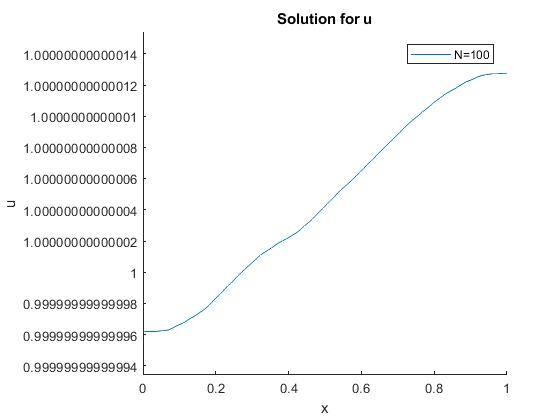
\includegraphics[width=150mm]{1Df1.jpg}
	\caption{showing the calculated u versus x, with N = 100,f(x)=1 \label{overflow}}
\end{figure}
\newpage

Figure 1.1 shows the solution for $u=\vec{f}/S$ for $N=100$ and $f(x)=1$. The domain is divided by equal spaced elements(follows from $f(x)=1$). Even though it is not a very stable or smooth curve, the solution does meet the requirement for the boundary condition where $du/dx=0$ at $x=0$ and $x=1$.

\section{Solution for u}
The final step is to combine all the codes in a main code to solve $Su= \vec{f}$. This code can be found in Appendix A. Previously the S matrix and f vector were computed for $n = 100$. Now $u$ will be calculated for $f(x)=1$, $D=1$, $\lambda = 1$ and $N = 100$. The result of this is plotted in figure(1.2). 


\begin{figure}[ht!]
	\centering
	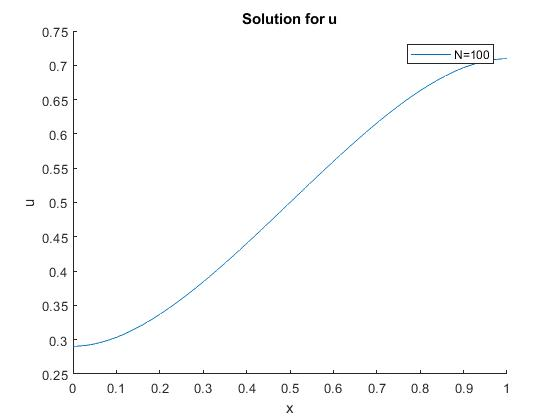
\includegraphics[width=140mm]{1Dfx.jpg}
	\caption{showing the calculated u versus x, with $N = 100$, $f(x)=x$		 \label{overflow}}
\end{figure}

Figure(1.2) shows the solution of $u=\frac{\vec{f}}{S}$ for $N=100$ elements. In this case f(x)=x is used as function to divide the elements. Compared to the case where f(x)=1 it can be seen that now a smoother curve is found. The solution found meets the requirement for the boundary condition where $du/dx=0$ at $x=0$ and $x=1$.

\vfill
\section{Experiment}

The next step is to see what happens when changing f(x) to $f(x)=sin(20x)$ and to see the difference for several values for N ($n=10,20,30,40,80,160)$.

\vspace{5mm}
\begin{lstlisting}
	function [f] = functionBVP(x)
		f = sin(20*x);
		%f = x;
		%f = 1;
	end
	
	figure 
	hold on
	
	for N_elem = [10 20 40 80 100 160]
	mesh = GenerateMesh(int,N_elem);
	elmat = GenerateTopology(N_elem);
	S = AssembleMatrix( N_elem, lambda, D, mesh, elmat);
	f = AssembleVector( N_elem, mesh, elmat);
	
	x = linspace(int(1),int(2),N_elem);
	
	u = S\f;
	plot(x,u);
	
	legend('N=100')
	title('Solution for u')
	xlabel('x')
	ylabel('u')
	ax.box='on'
	end
	hold off
\end{lstlisting}

\newpage

\begin{figure}[ht!]
	\centering
	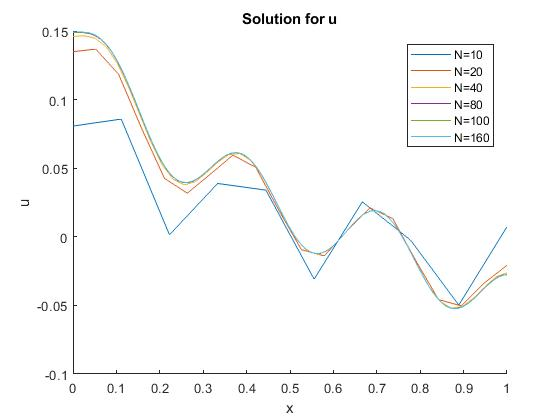
\includegraphics[width=150mm]{1Dfsinx.jpg}
	\caption{showing the calculated u versus x, with  $N =[10, 20, 40, 80, 100, 160],f(x)=sin(x)$. 
	\label{overflow}}
\end{figure}

Figure(1.3) shows the solution for u when picking $f(x)=sin(x)$. As the number of elements N is increased, it can be seen that an increasingly smooth line is drawn. The created MATLAB code divides the domain $x=[0,1]$ in N elements and then tries to solve the found equation while being consistent with the boundary condition. The boundary condition states that $du/dx =0$ at $x=0$ and $x=1$. For low numbers of N this is not achieved, but the higher number of elements shows that above $N=40$ the solution meets the boundary condition. Another thing one can observe is how the curve is similiar to a $sin(x)$, where a higher N value shows a better fit to a sinus.


\chapter{2D-case}


The obvious next step after solving a 1-dimensional BVP is to adept the 1D solutions and the created MATLAB code to solve a 2-dimensional BVP. To do this, a real life problem is now presented. In 3rd world countries one of the big issues is the supply of fresh water. One way is to do this is to take square reservoirs, which is a porous medium, with several wells where water is extracted from the subsurface. The water pressure is equal to the hydrostatic pressure. As this is not on an infinite domain, mixed boundary conditions are used. These boundary conditions represent a model for the transfer of the water over the boundary to locations far away. To this extent, a square domain is considered with length 2 in meter: $\Omega= (-1; 1) \times (-1; 1)$ with boundary $\partial\Omega$. Darcy's law for fluid determines the steady state equilibrium of this BVP, given by equation (2.1):

\begin{equation}
\vec{v}=-\frac{k}{\mu}\nabla p
\end{equation}
\medskip

Where $ p, k, \mu$ and $\vec{v}$, respectively denote the 
fluid pressure, permeability of the porous medium, viscosity of water and the fluid flow velocity. In this BVP the effect of gravity will not play a part as the problem is looked at in 2D. An accompanying assumption is incompressibility, so the extraction wells are treated as point sinks. This assumption can be made as the well its diameter is much smaller than the dimensions of the square reservoir. The extraction wells extract at the same rate in each direction, leading to the following boundary conditions (2.2).


\begin{equation}
	\nabla\cdot\vec{v}=-\sum_{p=1}^{n_{well}}Q_p\delta(\vec{x}-\vec{x}_p)=0,\quad (x,y) 	\in\Omega 
\end{equation}

Where $Q_p$ denotes the water extraction rate by well k, which is located at $x_p$. Here $x$ equals $(x;y)$, the spatial coordinates.  The convention $\vec{x} = (x; y) $ to represent the spatial coordinates is used. The dirac Delta Distribution is characterized by equation(2.3).

\begin{equation}
	\begin{cases} 
		\delta(\vec{x}) = 0,\quad  \vec{x} \neq 0 \\
		 \int\limits_{\Omega}\delta(\vec{x})d\Omega = 1, \quad $  where $\Omega $  contains the origin.$
	\end{cases} 
\end{equation}

\medskip

For this BVP the following boundary condition is considered: 

\begin{equation}
	\vec{v}\cdot\vec{n}=K(p-p^H), \quad (x,y) \in  \partial\Omega
\end{equation}
Where $K$ denotes the transfer rate coefficient of the water between the boundary of the domain and its surroundings. The constant $p^H$ represents the hydrostatic pressure. 

The boundary $\partial\Omega$ is divided into four parts described by the sides of the square domain $\Omega$. $\partial\Omega_1$ is the part with $x = -1$, $\partial\Omega_2$ is the part with $y = 1$, $\partial\Omega_3$ is the part with $x = 1$, $\partial\Omega_4$ is the part with $y = -1$.
\newpage

In order to solve this BVP the values needed for all the constants are given in table (2.1).


\begin{table}[h]
	\caption{Values of input parameters} % title of Table
	\centering % used for centering table
	\begin{tabular}{c c c} % centered columns (3 columns)
		\hline\hline %inserts double horizontal lines
		Symbol & Value & Unit\\ [0.5ex] % inserts table
		%heading
		\hline % inserts single horizontal line
		$Q_p$ & $50$ & $m^2/s$ \\ % inserting body of the table
		$k$ & $10^{-7}$ & $m^2$ \\
		$\mu$ & $1.002\cdot 10^{-3}$ & $Pa\cdot s$ \\
		$K$ & 10 & $m/s$ \\
		$p^H$ & $10^6$ & $Pa$ \\ [1ex] % [1ex] adds vertical space
		\hline %inserts single line
	\end{tabular}
	\label{table:nonlin} % is used to refer this table in the text
\end{table}
\bigskip

In this BVP six wells are considered, located at:


\begin{equation}
	\begin{cases} 
		x_p=0.6\cos(\frac{2\pi (p-1)}{5}) \\ x_p=0.6\sin(\frac{2\pi (p-1)}{5})
	\end{cases} 
\end{equation}

For $ p \in \{1, \dots ,5\}$ and for $p = 6$ we have $ x_6 = 0 $ and $ y_6 = 0 $.

\section{Boundary value problem 2D}
The first step to solving these equations using finite elements is to find the boundary value problem to solve. This is done by filling in equation(2.1) in both equation 2.2 and the boundary condition(2.4) in order to find the BVP in terms of p:
\vspace{5mm}


\begin{equation}
\text{BVP  }
	\begin{cases}
		-\frac{k}{\mu}\Delta\vec{p}=-\sum\limits_{p=1}^{n_{\text{well}}}Q_p\delta(\vec{x}-\vec{x}_p)=0,\, \, \quad (x,y) \, \in \, \Omega\\
		-\frac{k}{\mu}\nabla\vec{p}\cdot\vec{n}=-\frac{k}{\mu}\frac{\partial p}{\partial n} =K(p-p^H), \, \quad (x,y)\,  \in  \, \partial\Omega
	\end{cases}
\end{equation}

\bigskip

The next step is to compute the weak formulation using the previous found BVP(2.6). By multiplying both sides by test function $\phi(x) = \alpha_i + \beta_i x + \gamma_i y$ and integrating both sides over the domain $\Omega$ the weak formulation can be found.

\begin{equation}
	\int\limits_{\Omega}\phi(\vec{x})\nabla\cdot( -\frac{k}{\mu}\nabla\vec{p}) d\Omega =\int\limits_{\Omega}-\sum_{p=1}^{n_{well}}\phi(\vec{x})  Q_p\delta(\vec{x}-\vec{x}_p)d\Omega
\end{equation}

Using integrating by parts on the left side of equation(2.7) results in:
\begin{equation}
	\int\limits_{\Omega}\nabla\cdot \big[\phi(\vec{x})(-\frac{k}{\mu}\nabla\vec{p})] +\frac{k}{\mu}\nabla\phi(\vec{x})\cdot\nabla p d\Omega= -\int\limits_{\Omega}\sum_{p=1}^{n_{well}}\phi(\vec{x}) Q_p\delta(\vec{x}-\vec{x}_p)d\Omega
\end{equation}

Next is to apply Gauss's Theorem on the first term of the left side.
\begin{equation}
	\int\limits_{\partial\Omega}\vec{n}\cdot\big[\phi(\vec{x})(-\frac{k}{\mu}\nabla\vec{p})\big]d\tau+\int\limits_{\Omega}\frac{k}{\mu}\nabla\phi(\vec{x})\cdot\nabla p d\Omega= -\int\limits_{\Omega}\sum_{p=1}^{n_{well}}\phi(\vec{x}) Q_p\delta(\vec{x}-\vec{x}_p)d\Omega
\end{equation}


Switching the integral and summation on the right side of equation(2.9) and simplifying terms:

\begin{equation}
	\int\limits_{\partial\Omega}(\phi(\vec{x})(-\frac{k}{\mu}\frac{\partial\vec{p}}{\partial n}))d\tau+\int\limits_{\Omega}\frac{k}{\mu}\nabla\phi(\vec{x})\cdot\nabla p d\Omega= -\sum_{p=1}^{n_{well}}\int\limits_{\Omega}\phi(\vec{x}) Q_p\delta(\vec{x}-\vec{x}_p)d\Omega
\end{equation}


Equation(2.10) can be simplified, by using the boundary conditions (equation(2.6)) and the following property, into equation(2.12): 

\begin{equation}
	\int\limits_{\Omega}\delta(\vec{x})f(\vec{x})d\Omega \, = \, f(0)	
\end{equation}



\begin{equation}
	\int\limits_{\partial\Omega}\phi(\vec{x})K(p-p^H) d\tau+\int\limits_{\Omega}\frac{k}{\mu}\nabla\phi(\vec{x})\cdot\nabla p d\Omega= -\sum_{p=1}^{n_{\text{well}}}\phi(\vec{x}_p) Q_p
\end{equation}	

Rearranging equation(2.12) so that the unknowns are on the left and the constant parts on the right leads to the following WF:
\vspace{1mm}

 \begin{equation}
 \text{(WF)}
		\begin{cases} 
			$Find $p \in \sum =\{p$ $ smooth\}$ Such that:$ \\
			\int\limits_{\partial\Omega}\phi(\vec{x})Kp d\tau+\int\limits_{\Omega}\frac{k}{\mu}\nabla\phi(\vec{x})\cdot\nabla p d\Omega= -\sum\limits_{p=1}^{n_{well}}\phi(\vec{x}_p) Q_p +\int\limits_{\partial\Omega}\phi(\vec{x})Kp^Hd\tau\\ \forall\phi \in \sum 
		\end{cases}\  
\end{equation}
\vspace{1mm}

To solve the WF the Galerkin equations are applied, where $p$ is replaced by $ \sum\limits_{j=1}^{n}c_j\phi_j $ and  $\phi(x)=\phi_i(x)$.

\begin{equation}
	\sum\limits_{j=1}^{n}c_i\int\limits_{\partial\Omega}\phi_i K\phi_j d\tau + \int\limits_{\Omega}\frac{k}{\mu}\nabla\phi(x)\cdot\nabla \phi_j d\Omega= -\sum\limits_{p=1}^{n_{well}}\phi(x_p) Q_p +\int\limits_{\partial\Omega}\phi_i Kp^Hd\tau
\end{equation}

Equation(2.14) now is of the form $S\vec{c}=\vec{f}$ and, like with the 1D problem,  $\vec{c}$ can be computed. First the element and boundary elements are determined from the Galerkin equations.


\section{Element matrix and element vector}

First the galerkin equation is seperated in its element and boundary components. The element matrix $S^{e_k}_{ij}$ and the element vector $f^{e_k}_i$ are given in equations (2.15) and 2.16 respectively. For the element matrix, boundary element matrix and boundary element vector Newton-Côtes theorem and Holand-Bell theorem are applied to simplify the equations into a set of equations that can be used for computing with MATLAB code.

\begin{equation}
	S^{e_k}_{ij} = \int\limits_{e_k}\frac{k}{\mu}\nabla\phi_i\cdot\nabla \phi_j d\Omega = (\beta_i\beta_j+\gamma_i\gamma_j)\frac{k}{\mu}\frac{\lvert\triangle e_k\rvert}{2}
\end{equation}

\begin{equation}\label{f_i_ek}
	f^{e_k}_i =  -\sum_{p=1}^{n_{\text{well}}}\phi_i(\vec{x}_p) Q_p
\end{equation}


\section{Boundary matrix and boundary vector}

The boundary matrix $S^{be_l}_{ij}$ and boundary vector $f^{be_l}_i$ can be found in the following equations:

\begin{equation}
	S^{be_l}_{ij} = \int\limits_{be_l} K\phi_i \phi_j dx = K\frac{\lvert be_l\rvert}{6}(1+\delta_{ij})
\end{equation}

\begin{equation}
	f^{be_l}_i = Kp^H\int\limits_{be_l}\phi_i dx = K p^H \frac{\lvert be_l\rvert}{2}
\end{equation}
Where $\delta_{ij}$ is the Kronicker delta. It is assumed there are no wells on the boundary.

\section{Wells within an internal element}

To solve the BVP in 2D, one of the aspects that need to be determined is whether each internal element contains a well. So it must be determined whether the well with index $p$ and position $x_p$ is contained within element $e_k$ with vertices $x_{k1}$, $x_{k2}$ and $x_{k3}$. 

This can be done according the following criterion:

\begin{equation}
|\Delta(\vec{x}_p,\vec{x}_{k2},\vec{x}_{k3})|+|\Delta(\vec{x}_{k1},\vec{x}_p,\vec{x}_{k3})|+|\Delta(\vec{x}_{k1},\vec{x}_{x2},\vec{x}_p):
	\begin{cases} 
	=|e_k|,\, \vec{x}_p\, \in, \vec{e}_k\\ 
	>|e_k|,\, \vec{x}_p\, \notin\,\vec{e}_k
	\end{cases} 
\end{equation}

In the criterion $\Delta(\vec{x}_p,\vec{x}_q,\vec{x}_r)$ denotes the triangle with vertices $\vec{x}_p$, $\vec{x}_q$ and $\vec{x}_r$, where $|\Delta(\vec{x}_{k1},\vec{x}_{k2},\vec{x}_{k3})|$ denote its area. The triangular element $k$ is given by $e_k=\Delta(\vec{x}_{k1},\vec{x}_{k2},\vec{x}_{k3})$ with vertices  $\vec{x}_{k1}$, $\vec{x}_{k2}$ and $\vec{x}_{k3}$ and $\vec{e_k}$ includes the boundary of element $e_k$. To solve this BVP a certain tolerance has to be accounted for in the MATLAB code. However, while using this method it proved difficult to determine a correct tolerance to ensure every well was contained in a single element.

Therefore, an alternative method was used. A check was done whether the linear basis functions $\phi_{k1}$, $\phi_{k2}$ and $\phi_{k3}$ all have values in the interval $ [0,1] $ at position $\vec{x}_p$. If this is true, then the well at $\vec{x}_p$ is within the triangular element $e_k$.

If it is found that an element does contain a well, we see in equation \eqref{f_i_ek} that $\phi_i(\vec{x_p})$ for $i = \{k1, k2, k3\}$ must be found. The following code does this by determining $\alpha_i$, $\beta_i$, and $\gamma_i $ and subsequently filling $\vec{x}_p$ into the found $\phi_i(\vec{x})$.

\begin{lstlisting}
for index1=1:topology
	xc(index1) = x(elmat(i,index1));
	yc(index1) = y(elmat(i,index1));
end;

Delta = det([1 xc(1) yc(1);1 xc(2) yc(2);1 xc(3) yc(3)]);

B_mat = [1 xc(1) yc(1);1 xc(2) yc(2);1 xc(3) yc(3)] \  eye(3);

alpha = B_mat(1,1:3);
beta  = B_mat(2,1:3);
gamma = B_mat(3,1:3);

felem = zeros(1,topology);

if ~exist('u','var')  % Only if u is already know can the calculation of the velocity begin.
	for N = 1:N_wells
		for index3 = 1:topology
			phi_p(index3) = alpha(index3) + beta(index3)*xp(N) + gamma(index3)*yp(N);
		end
		if (phi_p(1) <= 1) && (phi_p(1) >= 0) && (phi_p(2) <= 1) && (phi_p(2) >= 0) && (phi_p(3) <= 1) && (phi_p(3) >= 0);
			for index1 = 1:topology
				felem(index1) = felem(index1) + -Qp*phi_p(index1); 
			end

		end
end


\end{lstlisting}


\section{Generating MATLAB code}

Similar as with the 1D BVP, MATLAB code is written in order to generate a mesh, element matrix, element vector, boundary element matrix and boundary element vector. These codes can be found in appendix B.1 through B.6. The scripts have been written such that they can be used to find both the pressure field and the velocity field(the derivation fort the velocities is found in the next section).

%Using the MATLAB codes a nice mesh can be found. ???

\begin{figure}[h]
	\centering
	\includegraphics[width=150mm]{meshgrid2D.jpg}
	\caption{Triangle element mesh over the square reservoir domain $\Omega=(-1;1)\times (-1;1)$. \label{overflow}}
\end{figure}




\section{Velocities}

In order to find the velocities in x,y-direction, Darcy's law is used to compute the speed in both directions.

%\begin{equation}
% M\vec{v_x}=C_x\vec{p},\,\,\, M\vec{v_y}=C_y\vec{p}
%\end{equation}

In order to find $v_x$ and $v_y$ the first step is to rewrite equation(2.20).

\begin{equation}
\vec{v}=-\frac{k}{\mu}\nabla p
\end{equation}

\begin{equation}
v_x=-\frac{k}{\mu}\frac{\partial p}{\partial x}
\end{equation}


\begin{equation}
v_y=-\frac{k}{\mu}\frac{\partial p}{\partial y}
\end{equation}

Equation(2.24) shows the relation between $\vec{v}$ and pressure p.

\begin{equation}
\vec{v}\cdot\vec{n}=k(p-p^H)\text{ on }\partial\Omega
\end{equation}

This relation gives the boundary conditions for $v_x$ and $v_y$:

\begin{equation}
v_x(x=-1)=-k(p-p^H)
\end{equation}


\begin{equation}
v_x(x=1)=k(p-p^H)
\end{equation}


\begin{equation}
v_y(y=-1)=-k(p-p^H)
\end{equation}


\begin{equation}
v_y(y=1)=k(p-p^H)
\end{equation}

%The Galerkin approach is used again to solve the equations by approximating $v_x$.
%
%\begin{equation}
%v_x \approx v^{(n)}_x=\sum_{j=1}^{n}c_j \phi_j
%\end{equation}
%
%Here $\phi (\vec{x})=\phi_i (\vec{x})$. Filling equations(2.29) and $\phi_i (\vec{x})$ in the exuations for $v_x$ 
In order to find the weak form, again, the test function $\phi$ and integration over the domain $\Omega$ is used. Here follows the derivation for finding $v_x$, the steps for deriving $v_y$ are similar.

\begin{equation}
\int\limits_{\Omega}\phi v_x d\Omega=-\frac{k}{\mu}\int\limits_{\Omega}\phi\frac{\partial p}{\partial x}d\Omega
\end{equation}

Partial integration is applied on the right side term.
\begin{equation}
\int\limits_{\Omega}\phi v_x d\Omega=  -\frac{k}{\mu}\{\int\limits_{\Omega}\frac{\partial }{\partial x}(\phi p)-p\frac{\partial \phi}{\partial x}d\Omega\}
\end{equation}

Rewriting the integral:

\begin{equation}
 \int\limits_{\Omega}-\frac{k}{\mu}\frac{\partial \phi p}{\partial x}dxdy=\int\limits_{-1}^{1}-\frac{k}{\mu}[\phi p]^{1}_{-1}dy
\end{equation}

The surface integral turns into a set of line integrals along parts of the boundary $\partial\Omega$.
\begin{equation}
\int\limits_{\Omega}-\frac{k}{\mu}\frac{\partial \phi p}{\partial x}dxdy=  \int\limits_{-1}^{1}-\frac{k}{\mu}(\phi(x=1,y)p(x=1,y))+\frac{k}{\mu}(\phi(x=-1)p(x=-1,y))dy
\end{equation}

Simplifying the previous equations.

\begin{equation}
\int\limits_{\Omega}-\frac{k}{\mu}\frac{\partial \phi p}{\partial x}dxdy =\int\limits_{\partial\Omega_3}-\frac{k}{\mu}\phi pd\tau+\int\limits_{\partial\Omega_1}\frac{k}{\mu}\phi pd\tau
\end{equation}

Inserting this into equation(2.29) the following equation is found.

\begin{equation}
	\int\limits_{\Omega}\phi v_x = \frac{k}{\mu}\{\int\limits_{\partial\Omega_3}-\phi pd\tau+\int\limits_{\partial\Omega_1}\phi pd\tau+\int\limits_{\Omega}p\frac{\partial \phi}{\partial x}d\Omega\}
\end{equation}

The boundary conditions is used to rewrite $p$ in the two boundary integrals.

%\begin{equation}
%\phi(\vec{x})=\phi_i(\vec{x}) \hspace{1cm}v_x\approx v^{(n)}_x = \sum_{j=1}^{n}c_j\phi_j(\vec{x})
%\end{equation}


\begin{equation}
\text{on}\,
\begin{cases}
\partial\Omega_3:\, -v_x=K(p-p^H) \,\rightarrow\, p=-\frac{v_x}{K}+p^H\\
\partial\Omega_1:\,\,\,\,\, v_x=K(p-p^H) \,\rightarrow\, p=\frac{v_x}{K}+p^H
\end{cases}
\end{equation}

The following weakform is derived:

%Now writing the equation where $v_x$ is filled in so that an equation is found that depends on $p$.

\vspace{1mm}

\begin{equation}
\text{WF}
	\begin{cases}
	$ Find $v_x \in \Sigma = \{v_x \text{ smooth}\}$, such that$ \\
		\int\limits_{\Omega}\phi v_x d\Omega + \int\limits_{\partial \Omega_3}-\frac{k}{\mu}\frac{1}{K}\phi v_xd\tau + \int\limits_{\partial \Omega_1}-\frac{k}{\mu}\frac{1}{K}\phi v_x d\tau 
		= \int\limits_{\partial \Omega_3}-\frac{k}{\mu}\phi p^H d\tau +\int\limits_{\partial \Omega_1}\frac{k}{\mu}\phi p^H d\tau + \int\limits_{\Omega}\frac{k}{\mu}p\frac{\partial \phi}{\partial x}d\Omega \\
		\forall \phi \in \Sigma
	\end{cases}
\end{equation}

\vspace{1mm}

To find the system of equations the following equations are filled in equation(2.35)  
$\phi(\vec{x})=\phi_i(\vec{x})= \alpha_i+\beta_i x+\gamma_i y$ and  $v_x\approx \sum\limits_{j=1}^{n}c_j\phi_j(\vec{x})$.

\begin{equation}\label{SoQ2}
	\sum_{j=1}^{n}c_j\{\int\limits_{\Omega}\phi_i\phi_j d\Omega +\int\limits_{\partial\Omega_3}-\frac{k}{\mu}\frac{1}{k}\phi_i\phi_j d\tau + \int\limits_{\partial\Omega_1}-\frac{k}{\mu}\frac{1}{k}\phi_i\phi_j d\tau\} = \\
	\int\limits_{\partial\Omega_3}-\frac{k}{\mu}\phi_i p^H d\tau +\int\limits_{\partial\Omega_1}\frac{k}{\mu}\phi_i p^H d\tau + \int\limits_{\Omega}\frac{k}{\mu}p\beta_id\Omega 
\end{equation}

From this system of equations the element matrix and element vector are extracted.

\begin{equation}
S_{ij}=\int\limits_{\Omega}\phi_i\phi_j d\Omega +\int\limits_{\partial\Omega_3}-\frac{k}{\mu}\frac{1}{k}\phi_i\phi_j d\tau + \int\limits_{\partial\Omega_1}-\frac{k}{\mu}\frac{1}{k}\phi_i\phi_j d\tau 
\end{equation}

\begin{equation}
f_i = 
\int\limits_{\partial\Omega_3}-\frac{k}{\mu}\phi_i p^H d\tau +\int\limits_{\partial\Omega_1}\frac{k}{\mu}\phi_i p^H d\tau + \int\limits_{\Omega}\frac{k}{\mu}p\beta_id\Omega
\end{equation}

Now separating contributions to both $S_{ij}$ and $f_i$ from boundary and internal elements into $S_{ij}^{be_l}$, $S_{ij}^{e_k}$, $f_i^{be_l}$ and $f_i^{e_k}$ such that:

\begin{equation}
	S_{ij} = \sum\limits_{l=1}^{n_{be}} S_{ij}^{be_{l}} + \sum\limits_{k=1}^{n_{e}} S_{ij}^{e_{k}}
\end{equation}

\begin{equation}
f_{i} = \sum\limits_{l=1}^{n_{be}} f_{i}^{be_{l}} + \sum\limits_{k=1}^{n_{e}} f_{i}^{e_{k}}
\end{equation}

Applying Newton-Côtes theorem and Holand-Bell theorem results in the following new expressions for the (boundary) element-matrix and -vector are found.

\begin{equation}
S^{e_k}_{ij}=\int\limits_{e_k}\phi_i\phi_j d\Omega= \frac{\lvert\triangle e_k \rvert}{24}
\end{equation}

\begin{equation}
S^{be_l}_{ij}=\int\limits_{be_l}-\frac{k}{\mu}\phi_i\phi_j d\tau = \frac{k}{\mu}\frac{1}{k}\frac{\lvert be_l\rvert}{6}(1+\delta_{ij})
\end{equation}

\begin{equation}
f^{e_n}_{i} = \int\limits_{e_k}\frac{k}{\mu}p\beta_i d\Omega = \frac{k}{\mu}\beta_i\sum_{m=\in\{k_1,k_2,k_3\}} p(\vec{x}_m) \frac{\lvert \triangle e_k\rvert}{6}
\end{equation}

\begin{equation}
f^{be_l}_{i}=\int\limits_{be_l}\pm \frac{k}{\mu}\phi_ip^H d\tau = \pm \frac{k}{\mu}p^H \frac{\lvert be_l\rvert}{2}
\end{equation}
With '$+$' if $be_{l}$ is on $\partial\Omega_1$ and '$-$' if it is on $\partial\Omega_3$
\vspace{5mm}

Since the pressure field $p$ was previously calculated, all the necessary information to compute $v_x$ (and similarly $v_y$) is now derived. Therefore it is possible to now evaluate our square reservoir. In the following plots the velocities for $K=10\,m/s$ that are computed are shown using a vector plot, contour plot and a 3D surface plot.\par In figure 2.2, 2.3 and 2.4 it can be seen that there are 6 spots that stick out: these are the wells. Looking at the velocity field, it can be seen that the velocity is highest around the wells and lowest near the boundaries. The heat contour plot implies that where the velocity is highest, the pressure is lowest in the square reservoir and at the boundary the highest pressure. The last figure shows a surface plot in accordance to the velocity field and pressure contour plot. Where the pressure difference is highest, one would expect the velocty to be highest. Velocity depends on pressure by the following relation: $\vec{v}=-\frac{k}{\mu}\nabla p$. At the peaks the gradient of $p$ is largest and results in a higher velocityS.



\begin{figure}[ht!]
	\centering
	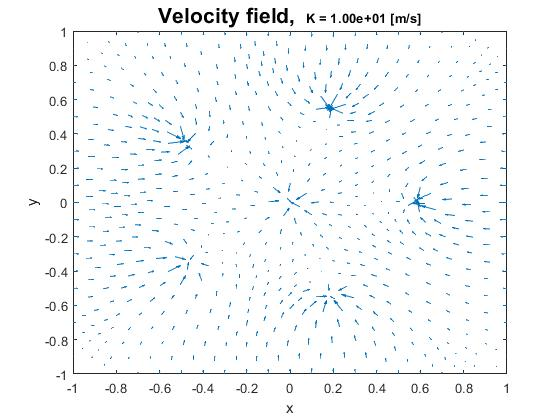
\includegraphics[width=130mm]{2Dvarrowsk10.jpg}
	\caption{Arrow velocity plot, indicating the direction and velocity of the water(longer arrows indicate higher velocity).
	\label{overflow}}
\end{figure}

\begin{figure}
	\centering
	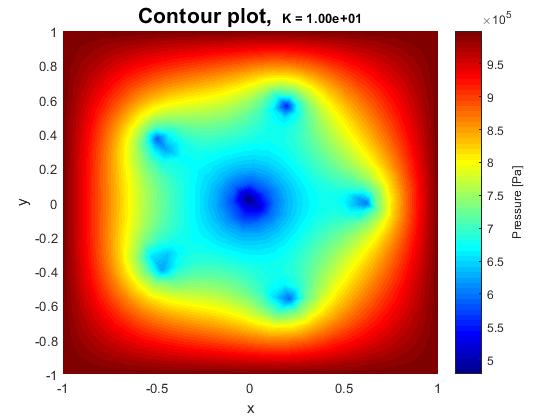
\includegraphics[width=130mm]{2Dvheatk10.jpg}
	\caption{Contour plot of the velocity in the square reservoir on domain $\Omega=(-1,1)\times(-1,1)$, showing six areas(the wells) where a drop of about two times the pressure can be observed, compared to the boundary pressure.
	\label{overflow}}
\end{figure}

\begin{figure}
	\centering
	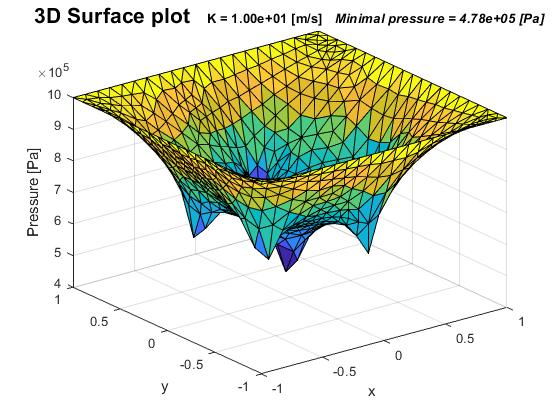
\includegraphics[width=130mm]{3Dvk10.jpg}
	\caption{3D surface plot for $K=10$. The lowest peaks indicate where the pressure is at a minimum in the square water reservoir.
	\label{overflow}}
\end{figure}


\newpage
\section{Varying constant $K$}

Now that the velocities have been calculated the last thing to vary is, is the factor $K$, the transfer rate coefficient of the water between the boundary of the domain and its surroundings. A few different plots will now follow in which the transfer coefficient $K$ has different values between 0.00001 and 10000. These plots can be found on the next page(figure 2.5). Looking at the plots it can be seen that the plots become increasinly darker as the $K$ factor increases. The pressure around the wells, where the pressure is at its minimum, also increases. When the $K$ factor is above $K=1$ the contour plots become similar. From an engineering point of view one could state that this means that a certain treshold $(K>x)$ has to be achieved, with $x$ being the minimum value at which the pressure profile shows enough pressure at the wells. If this treshold is not met the water will dissipate horizontaly in the reservoir instead of being pushed out through the well. The weight of the water due to the effect of gravity has to be overcome by the pressure of the reservoir.\\

\begin{figure}
	\centering
	\begin{subfigure}{.45\textwidth}
		\centering
		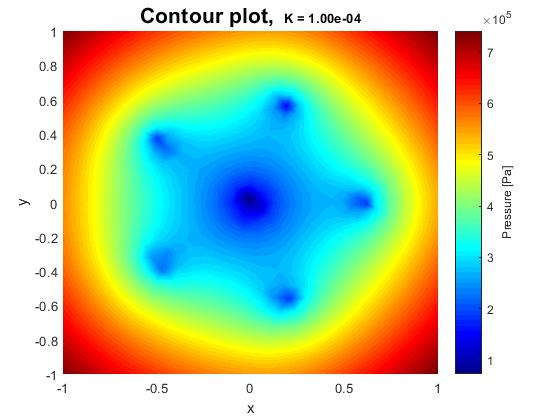
\includegraphics[width=8cm]{2Dheatk00001.jpg}
		\caption{$K=0.0001$}
		\label{fig:sub1}
	\end{subfigure}%
	\begin{subfigure}{.45\textwidth}
		\centering
		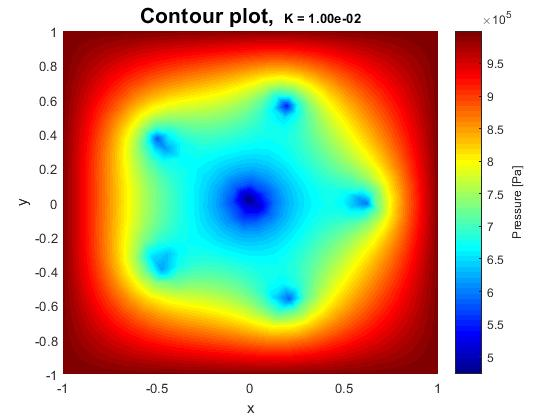
\includegraphics[width=8cm]{2Dheatk001.jpg}
		\caption{$K=0.001$}
		\label{fig:sub2}
	\end{subfigure}
	\begin{subfigure}{.45\textwidth}
	\centering\
	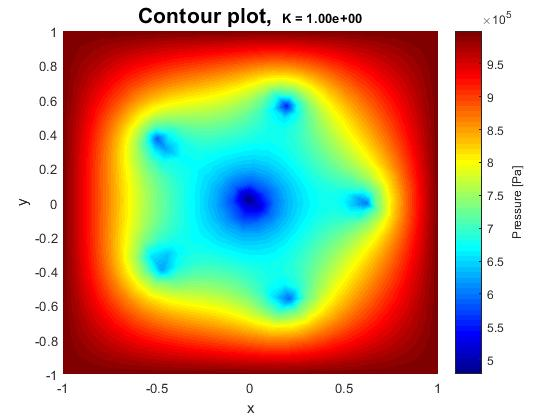
\includegraphics[width=8cm]{2Dheatk1.jpg}
	\caption{A subfigure}
	\label{fig:sub3}
	\end{subfigure}%
	\begin{subfigure}{.45\textwidth}
	\centering
	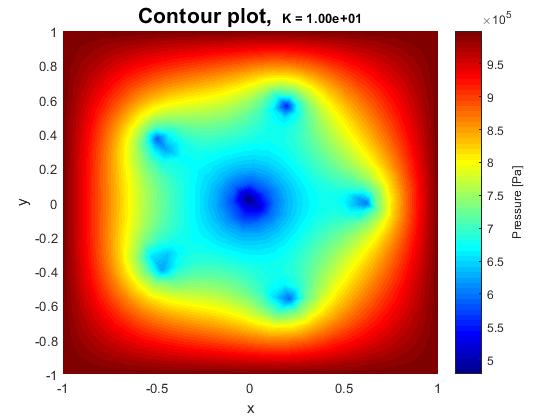
\includegraphics[width=8cm]{2Dvheatk10.jpg}
	\caption{$K=10$}
	\label{fig:sub4}
\end{subfigure}
	\begin{subfigure}{.45\textwidth}
	\centering\
	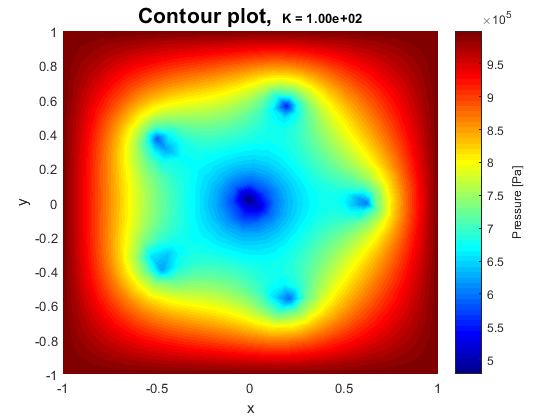
\includegraphics[width=8cm]{2Dheatk100.jpg}
	\caption{$K=100$}
	\label{fig:sub3}
\end{subfigure}%
\begin{subfigure}{.45\textwidth}
	\centering
	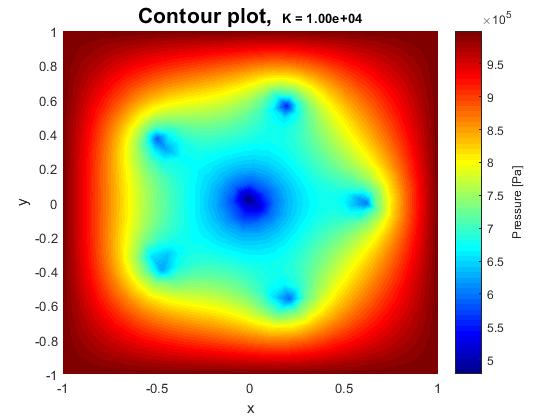
\includegraphics[width=8cm]{2Dheatk10000.jpg}
	\caption{$K=1000$}
	\label{fig:sub4}
\end{subfigure}
	\caption{A figure with two subfigures}
	\label{fig:test}
\end{figure}




The final step is to determine what happens when $K=0$ and why? When looking at our previous plots, when varying $K$ from 0.00001 to 10000 it can be derived that the pressure drops the lower the value for K is. This would mean that when $K=0$, the transfer coefficient of the water between the boundary of the square reservoir and its surroundings is zero. There will be no flow from the square reservoir into the surrounding through the wells. For engineering purpose designing a square reservoir such that it has a K value and therefore no flow, is an unwanted feature. The purpose of calculating the pressure is to make sure there is enough pressure present in the reservoir for water to flow up the wells.


\newpage
\chapter{Conclusion}

This report was written in order to better understand and demonstrate the application of finite elements in combination with MATLAB. This was shown by considering two boundary value problems: a 1D-case and a 2D-case. In the 1D-case a general BVP with boundary conditions were used to show how to solve this BVP. From the 1D-case it was derived that depending on how many $N$ and the chosen function $f(x)= function$ can greatly change the outcome of your solution. More elements(higher N) will result in a smoother graph. The function $f(x)= function$ was changed from $f(x)=1$ to $f(x)=x$ to $f(x)=sin(x)$. The graphs showed the solution curves became increasingly smoother.\par
In the 2D-case a real life problem was presented. The 2D BVP solved was an underground square reservoir with six wells through which water is extracted from the subsurface. Applying finite elements to solve this BVP and then adapting the MATLAB code used in the 1D-case it was possible to create velocity field plots and heat contour and 3D surface contour plots of the pressure $P$. From these plots it was derived that at the wells a decrease of pressure and increase of velocity is observed. The height of the pressure and velocity depends on the $K$ factor, the transfer rate coefficient by which the water flows from the reservoir to its surroundings. From the heat contour plots it was concluded that the pressure the overall pressure increases as the $K$ factor is increased. When the $K$ factor is too low, a heat contour plot is observed that could indicate that the pressure is too low at the wells for water to flow through the wells and instead will dissipate in the reservoir. At $K=0$ it is expected that the pressure is equal everywhere in the reservoir and no transfer flow is possible. From an engineering point it is thus necessary that the $K$ factor is above a certain treshold that allows water to flow through the well, with high enough pressure to counteract the gravity.  











\appendix

\begin{appendices}
\chapter{1D-case}

\section{Script}
\begin{lstlisting}
clear all
close all

%%Finite Element 1D
%% Parameters

N_elem = 100; %Number of elements
int = [0,1]; %Interval
lambda = 1;
D = .1;

%% Mesh & Topology

mesh = GenerateMesh(int,N_elem);
elmat = GenerateTopology(N_elem); %1D topology!!

%% Assemble Matrix & Vector

S = AssembleMatrix( N_elem, lambda, D, mesh, elmat);
f = AssembleVector( N_elem, mesh, elmat);

%% Calculate u
x = linspace(int(1),int(2),N_elem);

u = S\f;

hold on
plot(x,u); 
legend('N=100')
title('Solution for u')
xlabel('x')
ylabel('u')
ax.box='on'
hold off


% For this part change the function in functionBVP.m to 'f = sin(20*x)'

figure 
hold on

for N_elem = [10 20 40 80 100 160]
	mesh = GenerateMesh(int,N_elem);
	elmat = GenerateTopology(N_elem);
	S = AssembleMatrix( N_elem, lambda, D, mesh, elmat);
	f = AssembleVector( N_elem, mesh, elmat);

	x = linspace(int(1),int(2),N_elem);

	u = S\f;
	plot(x,u);


end

legend('N=10','N=20','N=40','N= 80','N=100','N=160')
title('Solution for u')
xlabel('x')
ylabel('u')
ax.box='on'
hold off





\end{lstlisting}

\section{Functions}

\begin{lstlisting}
function [ x ] = GenerateMesh(int, N_elem)
%GenerateMesh Creates a mesh for 1D problems
%   Detailed explanation goes here

x = linspace(int(1,1),int(1,2),N_elem);

end
\end{lstlisting}

\begin{lstlisting}
function [ elmat ] = GenerateTopology( N_elem )
%GenerateTopology Creates the topology for a 1D problem given mesh 'x'.
%   Detailed explanation goes here

elmat = zeros(N_elem,2);

for i = 1:N_elem-1
	elmat(i,1) = i;
	elmat(i,2) = i + 1;
end

end

\end{lstlisting}

\begin{lstlisting}
function [ S ] = AssembleMatrix( N_elem, lambda, D, mesh, elmat)
%AssembleMatrix Assembles matrix S from element matrix S_ek
%   Detailed explanation goes here

S = zeros(N_elem,N_elem);

for i = 1:N_elem-1
	Selem = GenerateElementMatrix(i, elmat, D, lambda, mesh);
	for j = 1:2
		for k = 1:2
			S(elmat(i,j), elmat(i,k)) = S(elmat(i,j), elmat(i,k)) + Selem(j,k);
		end
	end
end

end
\end{lstlisting}
\newpage
\begin{lstlisting}
function [ Selem ] = GenerateElementMatrix( k, elmat, D, lambda, mesh)
%GenerateElementMatrix Creates element matrix S_ek
%   Detailed explanation goes here

Selem = zeros(2,2);

i = elmat(k,1);
j = elmat(k,2);

x1 = mesh(i);
x2 = mesh(j);

element_length = abs(x1-x2);

slope = 1/element_length; 

for m = 1:2
	for n = 1:2
		if m == n
			Selem(m,n) = element_length*((-1)^(abs(m-n))*D*slope^2 + (2)*lambda/6);
			else
			Selem(m,n) = element_length*((-1)^(abs(m-n))*D*slope^2 + (1)*lambda/6);
		end
	end

end
end
\end{lstlisting}


\begin{lstlisting}
function [ f ] = AssembleVector( N_elem, mesh, elmat )
%AssembleVector Assembles vector f from element vector f_ek
%   Detailed explanation goes here

f = zeros(N_elem,1);

for i = 1:N_elem-1
	felem = GenerateElementVector(i, elmat, mesh);
	for j = 1:2
		f(elmat(i,j)) = f(elmat(i,j)) + felem(j);
	end
end
\end{lstlisting}

\begin{lstlisting}
function [ felem ] = GenerateElementVector( i, elmat, mesh )
%GenerateElementVector Creates element vector f_ek
%   Detailed explanation goes here

felem = [0;0];

k1 = elmat(i,1);
k2 = elmat(i,2);

x1 = mesh(k1);
x2 = mesh(k2);

element_length = abs(x1-x2);

felem = (element_length/2*arrayfun(@functionBVP,[x1,x2]))';

end
\end{lstlisting}

\chapter{2D-case}


\section{Generate mesh}
\begin{lstlisting}
clear all

Geometry = 'squareg'; 

DiffCoeff = 1;
h_transfer = 1;
u_inf = 1;


% Geometry = 'squareg'; % gives square [-1,1] x [-1,1]
% Geometry = 'circleg'; % gives unit circle centered at origin
% Geometry = 'lshapeg'; % gives L-shape

[p,e,t] = initmesh(Geometry);
[p,e,t] = refinemesh(Geometry,p,e,t); % gives gridrefinement
[p,e,t] = refinemesh(Geometry,p,e,t); % gives second gridrefinement
%[p,e,t] = refinemesh(Geometry,p,e,t); % gives third gridrefinement
pdemesh(p,e,t); % plots the geometry and mesh

x = p(1,:); y = p(2,:);
n = length(p(1,:));

elmat = t(1:3,:);
elmat = elmat';
elmatbnd = e(1:2,:);
elmatbnd = elmatbnd';
% h
topology = 3; topologybnd = 2;
\end{lstlisting}


\newpage

\section{Generate element matrix}
\begin{lstlisting}
clear xc
clear yc
clear Selem

for index1 = 1:topology
	xc(index1) = x(elmat(i,index1));
	yc(index1) = y(elmat(i,index1));
end;

Delta = det([1 xc(1) yc(1);1 xc(2) yc(2);1 xc(3) yc(3)]);
B_mat = [1 xc(1) yc(1);1 xc(2) yc(2);1 xc(3) yc(3)] \  eye(3);

alpha = B_mat(1,1:3);
beta  = B_mat(2,1:3);
gamma = B_mat(3,1:3);

for index1 = 1:topology
	for index2 = 1:topology
		if ~exist('u','var')
			Selem(index1,index2) =
			abs(Delta)/2*(k/mu)*(beta(index1)*beta(index2)+gamma(index1)*gamma(index2));
		else
			Selem(index1,index2) = abs(Delta)/24;
		end
	end;
end;
\end{lstlisting}
\newpage
\section{Generate element vector}
\begin{lstlisting}

% Module for element mass matrix for reactive term
%
% Output: felem  ====== vector of two components
%
% felem(1), felem(2) to be computed in this routine.

clear xc
clear yc
clear felem

for index1=1:topology
	xc(index1) = x(elmat(i,index1));
	yc(index1) = y(elmat(i,index1));
end;

Delta = det([1 xc(1) yc(1);1 xc(2) yc(2);1 xc(3) yc(3)]);

B_mat = [1 xc(1) yc(1);1 xc(2) yc(2);1 xc(3) yc(3)] \  eye(3);

alpha = B_mat(1,1:3);
beta  = B_mat(2,1:3);
gamma = B_mat(3,1:3);

felem = zeros(1,topology);

if ~exist('u','var')  % Only if u is already know can the calculation of the velocity begin.
	for N = 1:N_wells
		for index3 = 1:topology
			phi_p(index3) = alpha(index3) + beta(index3)*xp(N) + gamma(index3)*yp(N);
		end

		if (phi_p(1) <= 1) && (phi_p(1) >= 0) && (phi_p(2) <= 1) && (phi_p(2) >= 0) && (phi_p(3) <= 1) && (phi_p(3) >= 0);
			for index1 = 1:topology
				felem(index1) = felem(index1) + -Qp*phi_p(index1); 
			end

%         N_Test = N_Test + 1;

% Components of f are zero except for those elements with a well! So no
% other contributions!
%     else        
%         for index1 = 1:topology
%         global_index = elmat(N,index1);    
%         end
		end
	end
else
	switch direction
		case 1 % x direction
			for index1 = 1:topology
				felem(index1) = felem(index1) + (k/mu)*(abs(Delta)/6)*beta(index1)*(u(elmat(i,1))+u(elmat(i,2))+u(elmat(i,3)));
			end
		case 2 % y direction
			for index1 = 1:topology
				felem(index1) = felem(index1) + (k/mu)*(abs(Delta)/6)*gamma(index1)*(u(elmat(i,1))+u(elmat(i,2))+u(elmat(i,3)));
			end
	end
end


\end{lstlisting}



\newpage

\section{Generate Boundary element matrix}

\begin{lstlisting}
clear xc
clear yc
clear BMelem

for index1=1:topologybnd
	xc(index1) = x(elmatbnd(i,index1));
	yc(index1) = y(elmatbnd(i,index1));
end;

lek = sqrt((xc(2)-xc(1))^2 + (yc(2)-yc(1))^2);

for index1=1:topologybnd
	if ~exist('u', 'var')
		BMelem(index1,index1) = K*lek/2;  % NC used! not HB!!
	else

		BMelem(index1,index1) = -(k/(mu*K))*lek/6;
	end
end;
\end{lstlisting}



\section{Generate boundary element vector:}

\begin{lstlisting}
clear xc
clear yc
clear bfelem

for index1 = 1:topologybnd
	xc(index1) = x(elmatbnd(i,index1));
	yc(index1) = y(elmatbnd(i,index1));
end;

lek = sqrt((xc(2)-xc(1))^2+(yc(2)-yc(1))^2);

if ~exist('u','var')
	for index1 = 1:topologybnd
		bfelem(index1) = K*pH*lek/2*u_inf;   %what is u_inf?
	end;
else
	for index1 = 1:topologybnd
		bfelem(index1) = ((k*pH)/mu)*lek/2*u_inf;   %what is u_inf?
%         bfelem(index1) = -(k/mu)*lek/6*u(elmat(i,ind1));
	end
end
\end{lstlisting}

\section{Buildmatrices and vectors}

\begin{lstlisting}
% This routine constructs the large matrices and vector.
% The element matrices and vectors are also dealt with.
% First the internal element contributions
% First Initialisation of large discretisation matrix, right-hand side vector

% Treatment of the internal (triangular) elements

if ~exist('u', 'var')  

	S 		= sparse(n,n); % stiffness matrix
	f 		= zeros(n,1); % right-hand side vector

	for i = 1:length(elmat(:,1)) % for all internal elements
		GenerateElementMatrix; % Selem	
		for ind1 = 1:topology
			for ind2 = 1:topology
				S(elmat(i,ind1),elmat(i,ind2))	= S(elmat(i,ind1),elmat(i,ind2)) + Selem(ind1,ind2);
			end;
		end;

		GenerateElementVector; % felem
		for ind1 = 1:topology
			f(elmat(i,ind1)) = f(elmat(i,ind1)) + felem(ind1);
		end;
	end;

% Next the boundary contributions

	for i = 1:length(elmatbnd(:,1)); % for all boundary elements extension of mass matrix M and element vector f
	GenerateBoundaryElementMatrix; % BMelem
		for ind1 = 1:topologybnd
			for ind2 = 1:topologybnd
				S(elmatbnd(i,ind1),elmatbnd(i,ind2)) = S(elmatbnd(i,ind1),elmatbnd(i,ind2)) + BMelem(ind1,ind2);
			end;
		end;
		GenerateBoundaryElementVector; % bfelem   
		for ind1 = 1:topologybnd
			f(elmatbnd(i,ind1)) = f(elmatbnd(i,ind1)) + bfelem(ind1);
		end;
	end;

	else

	Sx 		= sparse(n,n); % stiffness matrix

	fx 		= zeros(n,1); % right-hand side vector

	left_nodes = find(p(1,:) == -1); 
	top_nodes = find(p(2,:) == 1);
	right_nodes = find(p(1,:) == 1);
	bottom_nodes = find(p(2,:) == -1);

	bnd1_nodes = ismember(elmatbnd,left_nodes);
	bnd1 = find(bnd1_nodes(:,1) == 1 & bnd1_nodes(:,2) == 1);

	bnd2_nodes = ismember(elmatbnd,top_nodes);
	bnd2 = find(bnd2_nodes(:,1) == 1 & bnd2_nodes(:,2) == 1);

	bnd3_nodes = ismember(elmatbnd,right_nodes);
	bnd3 = find(bnd3_nodes(:,1) == 1 & bnd3_nodes(:,2) == 1);
	
	bnd4_nodes = ismember(elmatbnd,bottom_nodes);
	bnd4 = find(bnd4_nodes(:,1) == 1 & bnd4_nodes(:,2) == 1);


	direction = 1;

	for i = 1:length(elmat(:,1)) % for all internal elements
		GenerateElementMatrix; % Selem	
		for ind1 = 1:topology
			for ind2 = 1:topology
				if elmat(i,ind1) == elmat(i,ind2)
					Sx(elmat(i,ind1),elmat(i,ind2))	= Sx(elmat(i,ind1),elmat(i,ind2)) + 2*Selem(ind1,ind2);
				else
					Sx(elmat(i,ind1),elmat(i,ind2))	= Sx(elmat(i,ind1),elmat(i,ind2)) + Selem(ind1,ind2);
				end
			end;
		end;
		GenerateElementVector; % felem
		for ind1 = 1:topology
			fx(elmat(i,ind1)) = fx(elmat(i,ind1)) + felem(ind1);
		end;
	end;

% Next the boundary contributions



	for j = 1:length(bnd1); % left boundary
		i = bnd1(j);
		GenerateBoundaryElementMatrix; % BMelem
		for ind1 = 1:topologybnd
			for ind2 = 1:topologybnd
				if elmatbnd(i,ind1) == elmatbnd(i,ind2)
					Sx(elmatbnd(i,ind1),elmatbnd(i,ind2)) = Sx(elmatbnd(i,ind1),elmatbnd(i,ind2)) + 2*BMelem(ind1,ind2);
				else
					Sx(elmatbnd(i,ind1),elmatbnd(i,ind2)) = Sx(elmatbnd(i,ind1),elmatbnd(i,ind2)) + BMelem(ind1,ind2);
				end;
			end
		end;
		GenerateBoundaryElementVector; % bfelem   
		for ind1 = 1:topologybnd
			fx(elmatbnd(i,ind1)) = fx(elmatbnd(i,ind1)) + bfelem(ind1);
		end;
	end;

	for j = 1:length(bnd3); % right boundary
		i = bnd3(j);
		GenerateBoundaryElementMatrix; % BMelem
		for ind1 = 1:topologybnd
			for ind2 = 1:topologybnd
				if elmatbnd(i,ind1) == elmatbnd(i,ind2)
					Sx(elmatbnd(i,ind1),elmatbnd(i,ind2)) = Sx(elmatbnd(i,ind1),elmatbnd(i,ind2)) + 2*BMelem(ind1,ind2);
				else
					Sx(elmatbnd(i,ind1),elmatbnd(i,ind2)) = Sx(elmatbnd(i,ind1),elmatbnd(i,ind2)) + BMelem(ind1,ind2);
				end;
			end
		end;
		GenerateBoundaryElementVector; % bfelem   
		for ind1 = 1:topologybnd
			fx(elmatbnd(i,ind1)) = fx(elmatbnd(i,ind1)) - bfelem(ind1);
		end;
	end;

	direction = 2;

	Sy 		= sparse(n,n); % stiffness matrix

	fy 		= zeros(n,1); % right-hand side vector

	for i = 1:length(elmat(:,1)) % for all internal elements
		GenerateElementMatrix; % Selem	
		for ind1 = 1:topology
			for ind2 = 1:topology
				if elmat(i,ind1) == elmat(i,ind2)
					Sy(elmat(i,ind1),elmat(i,ind2))	= Sy(elmat(i,ind1),elmat(i,ind2)) + 2*Selem(ind1,ind2);
				else
					Sy(elmat(i,ind1),elmat(i,ind2))	= Sy(elmat(i,ind1),elmat(i,ind2)) + Selem(ind1,ind2);
				end
			end;
		end;
		GenerateElementVector; % felem
		for ind1 = 1:topology
			fy(elmat(i,ind1)) = fy(elmat(i,ind1)) + felem(ind1);
		end;
	end;

% Next the boundary contributions



	for j = 1:length(bnd2); % left boundary
		i = bnd2(j);
		GenerateBoundaryElementMatrix; % BMelem
		for ind1 = 1:topologybnd
			for ind2 = 1:topologybnd
				if elmatbnd(i,ind1) == elmatbnd(i,ind2)
					Sy(elmatbnd(i,ind1),elmatbnd(i,ind2)) = Sy(elmatbnd(i,ind1),elmatbnd(i,ind2)) + 2*BMelem(ind1,ind2);
				else
					Sy(elmatbnd(i,ind1),elmatbnd(i,ind2)) = Sy(elmatbnd(i,ind1),elmatbnd(i,ind2)) + BMelem(ind1,ind2);
				end;
			end
		end;
		GenerateBoundaryElementVector; % bfelem   
		for ind1 = 1:topologybnd
			fy(elmatbnd(i,ind1)) = fy(elmatbnd(i,ind1)) - bfelem(ind1);
		end;
	end;

	for j = 1:length(bnd4); % right boundary
		i = bnd4(j);
		GenerateBoundaryElementMatrix; % BMelem
		for ind1 = 1:topologybnd
			for ind2 = 1:topologybnd
				if elmatbnd(i,ind1) == elmatbnd(i,ind2)
					Sy(elmatbnd(i,ind1),elmatbnd(i,ind2)) = Sy(elmatbnd(i,ind1),elmatbnd(i,ind2)) + 2*BMelem(ind1,ind2);
				else
					Sy(elmatbnd(i,ind1),elmatbnd(i,ind2)) = Sy(elmatbnd(i,ind1),elmatbnd(i,ind2)) + BMelem(ind1,ind2);
				end;
			end
		end;	
		GenerateBoundaryElementVector; % bfelem   
		for ind1 = 1:topologybnd
			fy(elmatbnd(i,ind1)) = fy(elmatbnd(i,ind1)) + bfelem(ind1);
		end;
	end;
end

\end{lstlisting}

\section{Compute u and $v_x$/$v_y$}


\begin{lstlisting}
% Construction of linear problem

BuildMatricesandVectors;

% Solution of linear problem

u = S \ f;

BuildMatricesandVectors;

vx = Sx \ fx;
vy = Sy \ fy;
\end{lstlisting}
\newpage
\section{Full script}
\begin{lstlisting}
close all
clear all

%% 2D Assignment
% Lab Assignment 7

%% Create Mesh
WI4243Mesh

%% Parameters

Qp = 50;            % [m^2/s]
k = 10^-7;          % [m^2]
mu = 1.002*10^-3;   % [Pa*s]
K = 10000;             % [m/s]
pH = 10^6;          % [Pa]
N_wells = 6;        % number of wells

epsilon1 = 0.03;
N_Test = 0;
%% Coordinates of wells

for i = 1:N_wells-1;
xp(i) = 0.6*cos((2*pi)*(i-1)/(N_wells-1));
yp(i) = 0.6*sin((2*pi)*(i-1)/(N_wells-1));
end

xp(N_wells) = 0;
yp(N_wells) = 0;
clear i;


%% Compute Problem
WI4243Comp

%% Post
hold on

figure(2);
ax.BoxStyle = 'full';
hold off
trisurf(elmat,x,y,u)
xlabel('x'); ylabel('y'); zlabel('Pressure [Pa]');
title(['\bf\fontsize{16}3D Surface plot  \fontsize{10} K = ' num2str(K,'%10.2e\n') ' [m/s]  \it Minimal pressure = ' num2str(min(u), '%10.2e\n') ' [Pa]']);

lgd = legend();
% title(lgd,['3D Surface plot, K = ' num2str(K) '\it Minimal pressure = ' num2str(Pressure_minimum)]);

% title( {'Title';'subtitle'} )

figure(3); 
trisurf(elmat,x,y,u);
xlabel('x'); ylabel('y');
title(['\bf\fontsize{16}Contour plot, \fontsize{10} K = ',num2str(K,'%10.2e\n')]);
view(2); shading interp; colormap jet; colorbar; set(gcf,'renderer','zbuffer')
h = colorbar; ylabel(h, 'Pressure [Pa]');


figure(4); quiver(x,y,vx',vy'); axis([-1 1 -1 1]);
xlabel('x'); ylabel('y');
title(['\bf\fontsize{16}Velocity field, \fontsize{10} K = ' num2str(K,'%10.2e\n') ' [m/s]']);
%% Velocity part
hold off

\end{lstlisting}

\end{appendices}

\end{document}




	